%% FEUP THESIS STYLE for LaTeX2e
%% how to use feupteses (portuguese version)
%%
%% FEUP, JCL & JCF, 31 Jul 2012
%%
%% PLEASE send improvements to jlopes at fe.up.pt and to jcf at fe.up.pt
%%

%%========================================
%% Commands: pdflatex tese
%%           bibtex tese
%%           makeindex tese (only if creating an index)
%%           pdflatex tese
%% Alternative:
%%          latexmk -pdf tese.tex
%%========================================

\documentclass[11pt,a4paper,twoside,openright]{report}

%% For iso-8859-1 (latin1), comment next line and uncomment the second line
\usepackage[utf8]{inputenc}

%\usepackage[latin1]{inputenc}

%% Portuguese version

%% MIEIC options
%\usepackage[portugues,mieic]{feupteses}
%\usepackage[portugues,mieic,juri]{feupteses}
%\usepackage[portugues,mieic,final]{feupteses}
%\usepackage[portugues,mieic,final,onpaper]{feupteses}

%% MIEEC options
%\usepackage[portugues,mieec]{feupteses}
%\usepackage[portugues,mieec,juri]{feupteses}
%\usepackage[portugues,mieec,final]{feupteses}
%\usepackage[portugues,mieec,final,onpaper]{feupteses}

%% For other degrees
\usepackage[mieec,juri]{feupteses} % you must define the degree bellow

%% Options: 
%% - portugues: titles, etc in portuguese
%% - onpaper: links are not shown (for paper versions)
%% - backrefs: include back references from bibliography to citation place

%% Uncomment to create an index (at the end of the document)
%\makeindex

%% Path to the figures directory
%% TIP: use folder ``figures'' to keep all your figures
\graphicspath{{figures/}}

%%----------------------------------------
%% TIP: if you want to define more macros, use an external file to keep them
%some macro definitions

% format
\newcommand{\class}[1]{{\normalfont\slshape #1\/}}

% entities
\newcommand{\Feup}{Faculdade de Engenharia da Universidade do Porto}


\newcommand{\svg}{\class{SVG}}
\newcommand{\scada}{\class{SCADA}}
\newcommand{\scadadms}{\class{SCADA/DMS}}

\usepackage{mypackages}


\addbibresource{myrefs.bib}
%%----------------------------------------

%%========================================
%% Start of document
%%========================================
\begin{document}

%%----------------------------------------
%% Information about the work
%%----------------------------------------
\title{Aplicação de técnicas de aprendizagem profunda estruturada para diagnóstico de funcionamento de centrais fotovoltaicas.}
\author{David da Silva Moreira Freire}

%% Comment next line if not necessary for degree name
\degree{Mestrado em Engenharia Eletrotécnica e Computadores}

%% Uncomment next line for date of submission
%\thesisdate{31 de julho de 2008}

%% Comment next line for copyright text if not used
%\copyrightnotice{David Freire, 2022/2023}

\supervisor{Supervisor}{Cláudio Domingos Martins Monteiro}

%% Uncomment next line if necessary
%\supervisor{Co-orientador}{Nome de Outro Orientador}

%% Uncomment committee stuff in the final version if used
%\committeetext{Aprovado em provas públicas pelo Júri:}
%\committeemember{Presidente}{Nome do presidente do júri}
%\committeemember{Arguente}{Nome do arguente do júri}
%\committeemember{Vogal}{Nome do vogal do júri}

%% Uncomment signature line in the final on paper version if used
%\signature

%% Specify cover logo (in folder ``figures'')
\logo{uporto-feup.pdf}
 
%% Uncomment next line for additional text below the author's name (front page)
%\additionalfronttext{Preparação da Dissertação}

%%----------------------------------------
%% Preliminary materials
%%----------------------------------------

% remove unnecessary \include{} commands
\begin{Prolog}
  \chapter*{Resumo}
%\addcontentsline{toc}{chapter}{Resumo}

Este documento ilustra o formato a usar em dissertações na \Feup.
São dados exemplos de margens, cabeçalhos, títulos, paginação, estilos
de índices, etc. 
São ainda dados exemplos de formatação de citações, figuras e tabelas,
equações, referências cruzadas, lista de referências e índices.
Este documento não pretende exemplificar conteúdos a usar. 
É usado o \emph{Loren Ipsum} para preencher a dissertação.

Lorem ipsum dolor sit amet, consectetuer adipiscing elit. Etiam vitae
quam sed mauris auctor porttitor. Mauris porta sem vitae arcu sagittis
facilisis. Proin sodales risus sit amet arcu. Quisque eu pede eu elit
pulvinar porttitor. Maecenas dignissim tincidunt dui. Pellentesque
habitant morbi tristique senectus et netus et malesuada fames ac
turpis egestas. Donec non augue sit amet nulla gravida
rutrum. Vestibulum ante ipsum primis in faucibus orci luctus et
ultrices posuere cubilia Curae; Nunc at nunc. Etiam egestas. 

Donec malesuada pede eget nunc. Fusce porttitor felis eget mi mattis
vestibulum. Pellentesque faucibus. Cras adipiscing dolor quis
mi. Quisque sagittis, justo sed dapibus pharetra, lectus velit
tincidunt eros, ac fermentum nulla velit vel sapien. Vestibulum sem
mauris, hendrerit non, feugiat ac, varius ornare, lectus. Praesent
urna tellus, euismod in, hendrerit sit amet, pretium vitae,
nisi. Proin nisl sem, ultrices eget, faucibus a, feugiat non,
purus. Etiam mi tortor, convallis quis, pharetra ut, consectetuer eu,
orci. Vivamus aliquet. Aenean mollis fringilla erat. Vivamus mollis,
purus at pellentesque faucibus, sapien lorem eleifend quam, mollis
luctus mi purus in dui. Maecenas volutpat mauris eu lectus. Morbi vel
risus et dolor bibendum malesuada. Donec feugiat tristique erat. Nam
porta auctor mi. Nulla purus. Nam aliquam. 


\chapter*{Abstract}
%\addcontentsline{toc}{chapter}{Abstract}

The increase in photovoltaic power plants has led to the need for effective
methods for detecting and addressing component faults, which can have
significant economic impacts. In this work, we will explore the current state of
fault detection and state estimation tools in the field of PV systems, with a
focus on understanding how these tools work and identifying their strengths and
limitations. We will also propose improvements to existing approaches or develop
a novel approach to address this issue. By examining the most successful tools
to date and offering new solutions, we aim to help PV plant operators improve
the reliability and efficiency of their systems. % the abstract
  \chapter*{Agradecimentos}
%\addcontentsline{toc}{chapter}{Agradecimentos}

Aliquam id dui. Nulla facilisi. Nullam ligula nunc, viverra a, iaculis
at, faucibus quis, sapien. Cum sociis natoque penatibus et magnis dis
parturient montes, nascetur ridiculus mus. Curabitur magna ligula,
ornare luctus, aliquam non, aliquet at, tortor. Donec iaculis nulla
sed eros. Sed felis. Nam lobortis libero. Pellentesque
odio. Suspendisse potenti. Morbi imperdiet rhoncus magna. Morbi
vestibulum interdum turpis. Pellentesque varius. Morbi nulla urna,
euismod in, molestie ac, placerat in, orci. 

Ut convallis. Suspendisse luctus pharetra sem. Sed sit amet mi in diam
luctus suscipit. Nulla facilisi. Integer commodo, turpis et semper
auctor, nisl ligula vestibulum erat, sed tempor lacus nibh at
turpis. Quisque vestibulum pulvinar justo. Class aptent taciti
sociosqu ad litora torquent per conubia nostra, per inceptos
himenaeos. Nam sed tellus vel tortor hendrerit pulvinar. Phasellus
eleifend, augue at mattis tincidunt, lorem lorem sodales arcu, id
volutpat risus est id neque. Phasellus egestas ante. Nam porttitor
justo sit amet urna. Suspendisse ligula nunc, mollis ac, elementum
non, venenatis ut, mauris. Mauris augue risus, tempus scelerisque,
rutrum quis, hendrerit at, nunc. Nulla posuere porta orci. Nulla dui. 

Fusce gravida placerat sem. Aenean ipsum diam, pharetra vitae, ornare
et, semper sit amet, nibh. Nam id tellus. Etiam ultrices. Praesent
gravida. Aliquam nec sapien. Morbi sagittis vulputate dolor. Donec
sapien lorem, laoreet egestas, pellentesque euismod, porta at,
sapien. Integer vitae lacus id dui convallis blandit. Mauris non
sem. Integer in velit eget lorem scelerisque vehicula. Etiam tincidunt
turpis ac nunc. Pellentesque a justo. Mauris faucibus quam id
eros. Cras pharetra. Fusce rutrum vulputate lorem. Cras pretium magna
in nisl. Integer ornare dui non pede. 

\vspace{10mm}
\flushleft{David Freire} % ? tem que ser o nome completo
  % the acknowledgments
  \cleardoublepage
\thispagestyle{plain}

\vspace*{8cm}

\begin{flushright}
   \textsl{``\\Genetic predispositions are only that: predispositions. \\
      It’s not a destiny written in stone. People have choices.''} \\
\vspace*{1.5cm}
            Dr. Jennifer Melfi, The Sopranos
\end{flushright}
    % initial quotation if desired
  \cleardoublepage
  \pdfbookmark[0]{Contents}{contents}
  \tableofcontents
  \cleardoublepage
  \pdfbookmark[0]{List of Figures}{figures}
  \listoffigures
  \cleardoublepage
  \pdfbookmark[0]{List of Tables}{tables}
  \listoftables
  \chapter*{Abreviaturas e Símbolos}
%\addcontentsline{toc}{chapter}{Abbreviations}
\chaptermark{ABREVIATURAS E SÍMBOLOS}

\begin{flushleft}
\begin{tabular}{l p{0.8\linewidth}}
PV      & Photovoltaic\\
DC      & Direct current\\
STC      & Standard Test Conditions\\
MCD      & Minimum Covariance Determinant\\
WWW      & \emph{World Wide Web}
\end{tabular}
\end{flushleft}

  % the list of abbreviations used
\end{Prolog}

%%----------------------------------------
%% Body
%%----------------------------------------

\StartBody

\chapter{Introduction} \label{chap:intro}

As a company becomes more reliant on the data it produces to drive its
decisions, data warehouses become core components for providing data for
analysis and reporting. To populate the data warehouse, one of the most common
procedures is the ETL (Extract, Transform and Load) process which involves:
extracting the data from multiple data sources; transforming the data; loading
the data into the appropriate format for consultation.

It is also well known that as companies become more data driven,
the challenges associated with dealing with large volumes of data becomes more
apparent as digital solutions start failing to respond, or are unable to respond
within appropriate time constraints. 

For this reason, a distributed architecture that resorts to microservices is a
common and efficient way to tackle the problem as it simplifies scaling based on
the system's needs, nullifies the single point of failure, and increases the
system's resilience. 

On the other hand, incorrectly implemented communication between microservices
can become a distributed solution's scalability bottleneck, as the microservice
components can become too coupled and increase the technical cost of making any
changes to the system.  This is where message brokers come in.  Instead of
having the components communicating with one another directly, the message
broker serves as an intermediary that asynchronously delivers the information
between components as it is requested by the interested parts. In short, the
message broker mediates the communication between data producers (entities that
send data to the broker) and data consumers (entities that request data from
the broker). 

\begin{figure}[htb!]
    \centering
    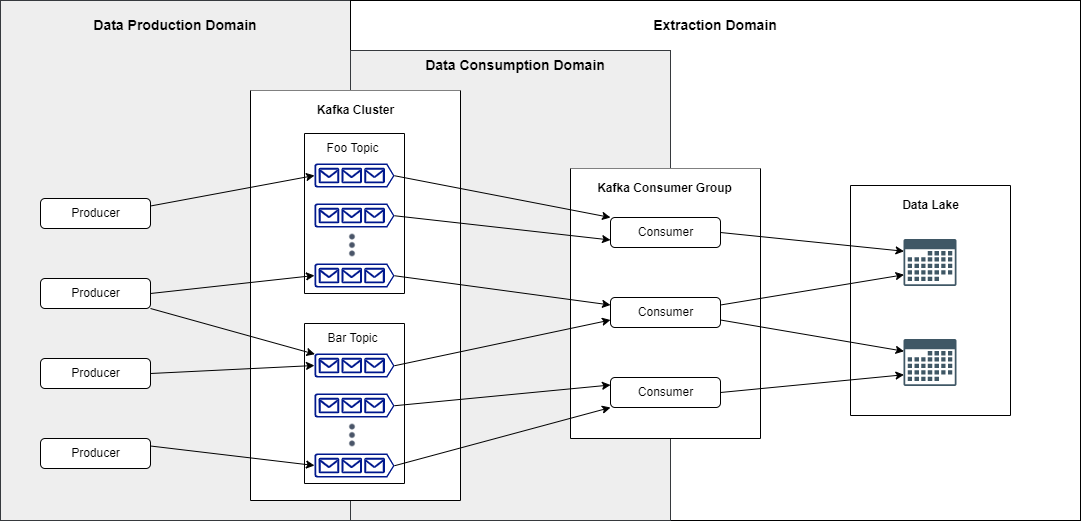
\includegraphics[width=\textwidth]{images/introduction/Context.png}
\caption{
    Data pipeline representing the flow of data since it is appended into one of
    the data sources (Topic), to when it is fetched by a consumer and inserted
    into a Data Lake.
}
\label{fig:problem_context}
\end{figure}

Throughout this work, we use Kafka as the message broker system. A Kafka cluster
is made of topics, which in turn is a unit that is subdivided into several logs,
commonly reffered to as partitions. When a producer sends a record to a specific
topic, it will be appended into one of the topic's partitions, illustrated in
the Data Production Domain in Figure \ref{fig:problem_context}. 

A consumer group is a unit composed of multiple consumers, each with the common
task of consuming data from the topics the group is subscribed to. To consume
the data within a topic, each of its partitions have to be assigned a single
consumer belonging to the same group. Assigning the partition's to different
consumers in a group, is Kafka's way of providing scalability. This design
feature leads to the fact that a group does not require more consumers than the
number of partitions, as only one consumer in a group can read data from a given
partition.

The problem was proposed by the data engineering team at HUUB (MAERSK), and it
is framed within the scope of the Extraction Domain in Figure
\ref{fig:problem_context}. It consists of being capable to dynamically manage a
group of consumers, to up- and down-scale the number of instances (i.e.
consumers), and also specify the tasks (partitions) that are assigned to each
consumer. We need to define the required amount of parallelism as to guarantee the
number of unread messages by the group does not increase with time. Hence, the
rate at which the group is consuming data from each partition, must be bigger or
equal to their respective write speed.

Considering consumers as bins, and partitions as items that have to be assigned
a bin, we model this problem as the Bin Packing Problem (BPP), with the
particularity that items vary in size with time. This occurs because the
partition's size correlates to its current write speed, which fluctuates based
on the current system's load and inevitably implies that a solution for a given
time instant may not hold true in future instants. 

On account of this BPP variation, a new solution has to be computed at each
instant, which might lead to a partition (item) being assigned to a different
consumer (bin) when compared to the consumer group's previous configuration.
Since two consumers cannot read from the same partition concurrently, the cost
associated to rebalancing a partition is related to the amount of data that is
not being read while the partition is being assigned to another consumer. 

Given that it is the first time the Bin Packing Problem is applied in this
context, existing algorithms do not take the rebalancing cost into account.
Hence, in Section \ref{sub:rscore} we propose a metric to account for a given
iteration's rebalance cost (Rscore). Additionally, using the Rscore, in Section
\ref{subsub:modified_any_fit} we propose four new BPP heuristic algorithms that
account for the rebalance costs.

The algorithms' performance is compared in section \ref{c3subsub:testing}. Since
the algorithms are attempting to solve a multi-objective problem that aims to
minimize both the number of bins required and the rebalance cost for a single
iteration, we compute the pareto front. It shows that three of the proposed
algorithms are a competitive solution to the problem at hand.

To deliver a fully automated solution to the autoscaling problem, in Chapter
\ref{chap:consumer_group_autoscaler} we introduce a system comprising three
components: a monitor, a consumer and a controller. Using the data from the
monitor process the controller uses the aforementioned theoretical approaches
(BBP heuristics) to assign tasks to consumers. Each of the components is
unitarily tested throughout Sections \ref{component:Monitor},
\ref{component:consumer} and \ref{component:controller}. An integration test is
also presented in Chapter \ref{chap:integration_tests}, aimed to reflect the
autoscaler's response time to the message broker's current load. Lastly, in
Chapter \ref{chap:conclusions}, we discuss results and suggest future work.
The following chapters introduce this thesis' technological and theoretical
background, Chapter \ref{chap:infrastructure} and Chapter \ref{chap:literature
review} respectively.


 


%% Comment next 2 commands if numbered appendices are not used
\appendix
\chapter{CellTAN Development}

\section{Statistical tests for measure of association} \label{ap1:stats}

\subsection{Pearson's chi squared test} \label{ap1:pearsonschi}

\begin{equation}
    \chi^2 = \sum_{i=1}^{k} \frac{(O_i - E_i)^2}{E_i}
\end{equation}
    
where:
\begin{align*}
\chi^2 & : \text{Chi-squared statistic} \\
O_i & : \text{Observed frequency for category } i \\
E_i & : \text{Expected frequency for category } i \\
k & : \text{Number of categories or cells in the data}
\end{align*}


\subsection{Fischer's exact test} \label{ap1:fischer}

\begin{equation}
    p = \frac{{\binom{a}{x} \binom{b}{y}}}{{\binom{N}{n}}}
\end{equation}

where:
\begin{align*}
    p & : \text{p-value of the test} \\
    a & : \text{Number of successes in group A} \\
    b & : \text{Number of successes in group B} \\
    x & : \text{Number of successes of interest in group A} \\
    y & : \text{Number of successes of interest in group B} \\
    N & : \text{Total number of observations} \\
    n & : \text{Number of observations in group A}
\end{align*}


\subsection{Odds ratio} \label{ap1:oddsratio}

\begin{equation}
OR = \frac{{a \cdot d}}{{b \cdot c}}
\end{equation}

where:
\begin{align*}
OR & : \text{Odds ratio} \\
a & : \text{Number of successes in group A} \\
b & : \text{Number of failures in group A} \\
c & : \text{Number of successes in group B} \\
d & : \text{Number of failures in group B}
\end{align*}

\subsection{Phi coefficient} \label{ap1:phi}

\begin{equation}
\phi = \sqrt{\frac{\chi^2}{N}}
\end{equation}

where:
\begin{align*}
\phi & : \text{Phi coefficient} \\
\chi^2 & : \text{Chi-squared statistic} \\
N & : \text{Total number of observations}
\end{align*}

\subsection{Contingency coefficient C} \label{ap1:contingencyc}

\begin{equation}
C = \sqrt{\frac{\chi^2}{N + \chi^2}}
\end{equation}

where:
\begin{align*}
C & : \text{Contigency coefficient} \\
\chi^2 & : \text{Chi-squared statistic} \\
N & : \text{Total number of observations}
\end{align*}


\subsection{Theil's U} \label{ap1:theilsu}

\begin{equation}
U(x|y) = \frac{H(x) - H(x|y)}{H(x)}
\end{equation}

Entropy of variable x:
\begin{equation}
H(x) = -\sum_{i=1}^{n} p(x_i) \log(p(x_i))
\end{equation}

Conditional entropy of variable x given variable y:
\begin{equation}
H(x|y) = -\sum_{i=1}^{n} \sum_{j=1}^{m} p(x_i, y_j) \log\left(\frac{p(x_i, y_j)}{p(y_j)}\right)
\end{equation}


\section{Technology stack} \label{ap1:techstack}

\begin{figure}[h!]
    \centering
    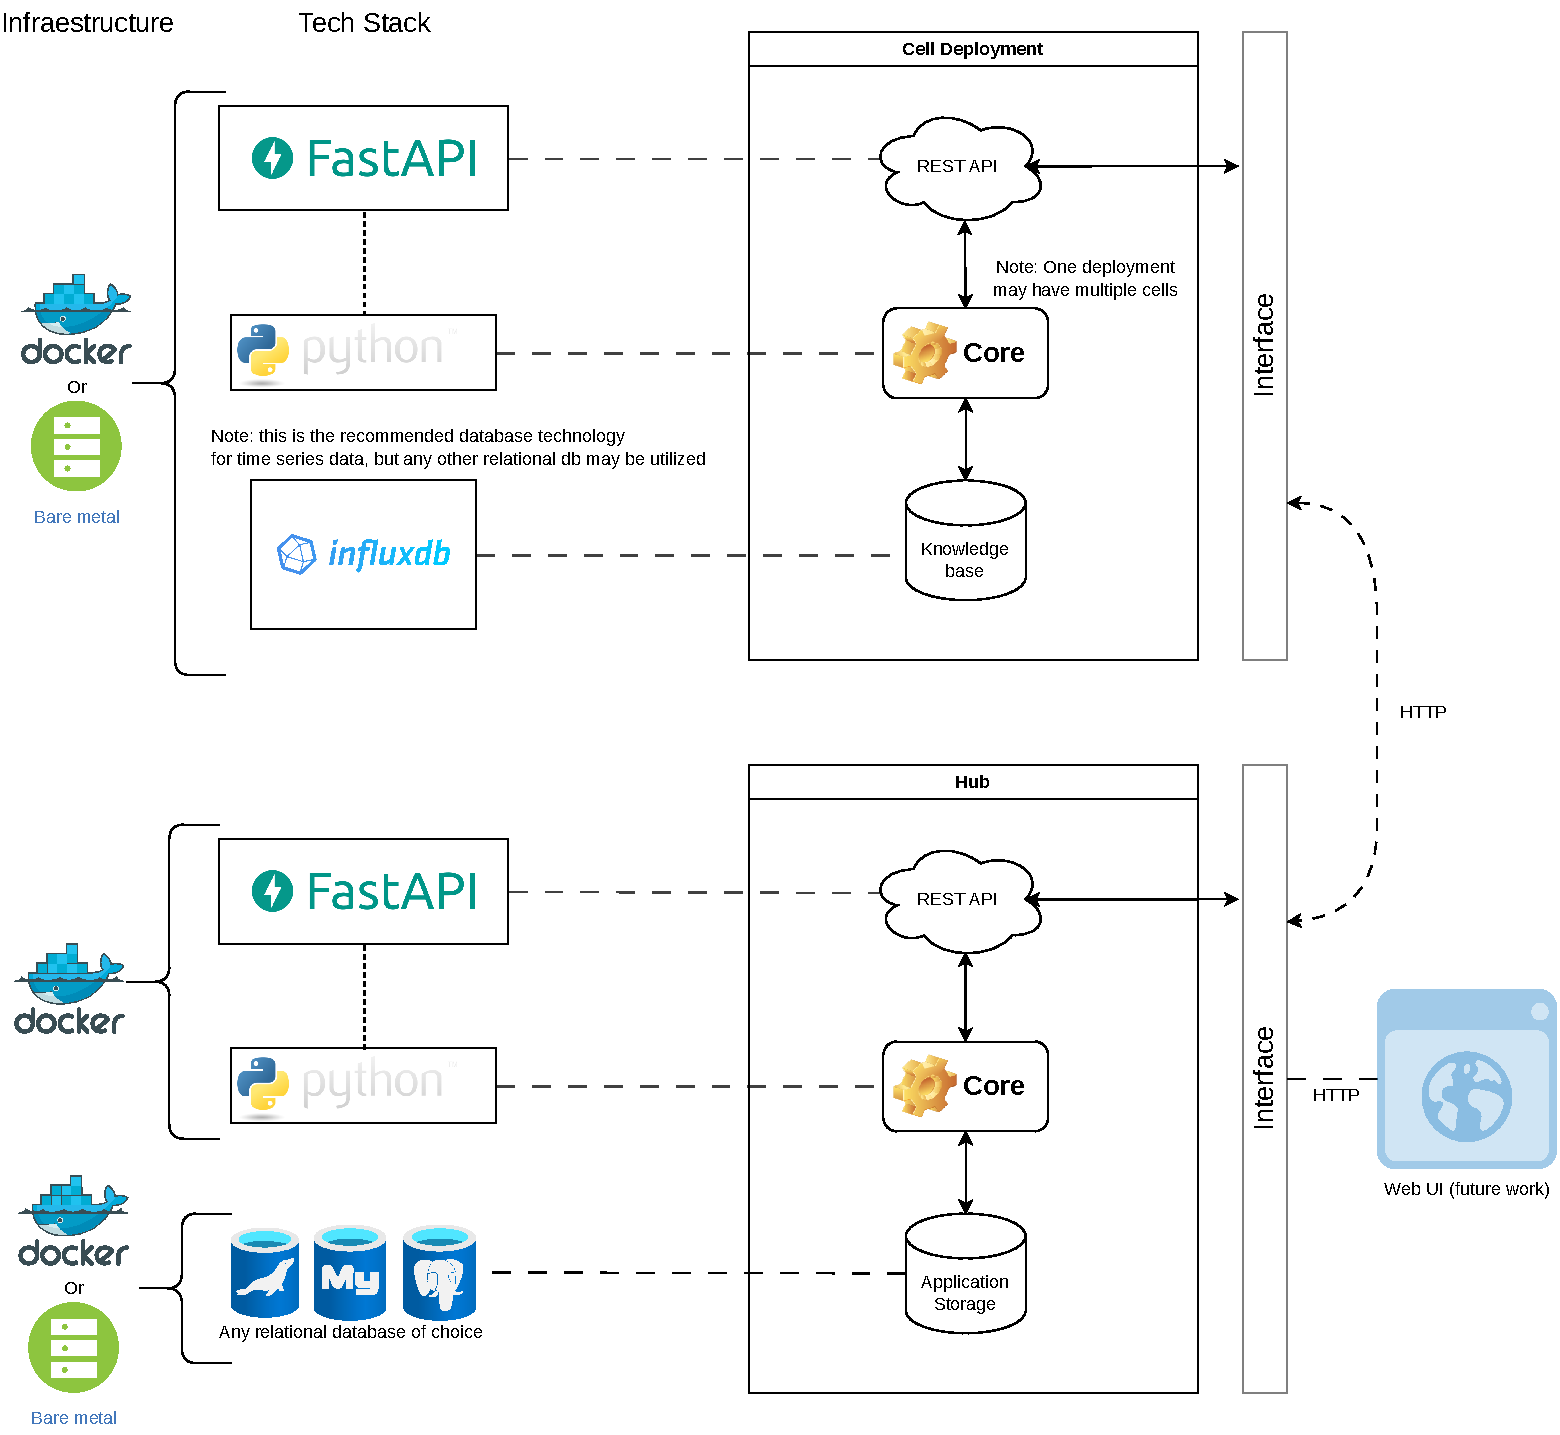
\includegraphics[width=\linewidth]{figures/appendix/a_development/techstack.pdf}
    \caption{Technology stack of the Cell and Hub of CellTAN.}
    \label{fig:techstack}
\end{figure}


\section{Cell configuration} \label{ap1:config}
 
% TODO overview da configuração da célula e ficheiro de configuração


\printbibliography

%% Index
%% Uncomment next command if index is required, 
%% don't forget to run ``makeindex tese'' command
%\PrintIndex
\end{document}
